As the system requires the use of moving parts, such as the conveyor belt and sweeper arm, there is a need to design electronics that can control these parts. For future reference, the following pins are connected to the following components:

\begin{table}[H]
    \centering
    {\fontsize{10pt}{12pt}\selectfont
    \begin{tabularx}{\textwidth}{|p{4cm}|p{4cm}|X|}
        \hline
        \textbf{Component} & \textbf{Pin} & \textbf{Description} \\
        \hline
        WS2812B LED Strip & GPIO10 & Controls the colour of the LEDs on the strip. \\
        \hline
        NEMA17 Stepper Motor (Conveyor Belt) & GPIO27 (DIR) \newline GPIO18 (STEP) & Controls the direction and steps of the motor. \\
        \hline
        NEMA17 Stepper Motor (Sweeper Arm) & GPIO6 (DIR) \newline GPIO3 (STEP) & Controls the direction and steps of the motor. \\
        \hline
        IR Break Beam Sensor & GPIO7 & Detects when a component is on the conveyor belt. \\
        \hline
        Limit Switch & GPIO17 & Detects when the sweeper arm is at its minimum position. \\
        \hline
        Okdo OV5647 Camera & CSI-2 & Captures images for the computer vision system. \\
        \hline
        LCD Display & HDMI \newline USB & Displays the user interface, powered directly from the Pi. \\
        \hline
    \end{tabularx}
    }
    \caption{Component Connections}
    \label{tab:component-connections}
\end{table}

\todo{show wiring diagram}

\subsubsection{Power Supply}

As mentioned in \autoref{sec:power-supply}, there are two XL4015 buck converters used to reduce the 24V output of the power supply to 5V and 12V. 18 AWG wire is used to both connect the 24V input to the buck converters, and to connect the output of the converters to the USB breakout boards. A standard 3-pin power cable connects the PSU's IEC C14 socket to the mains power.
\subsubsection{WS2812B LED Strip}
\label{sec:ws2812b-led-strip}
To illuminate the components on the conveyor belt, a WS2812B LED strip was used. It is powered with 5V, however it cannot be powered directly from the Pi due to the high current draw of the strip. Instead, a USB-C breakout board is connected to the 5V input pins, and then a USB-C cable is connected from the power supply to the breakout board, allowing the LED strip to be powered from the 5V output of the power supply. A USB hub is used to allow both the Pi and the LED strip to be powered from the same USB port on the power supply.

\begin{figure}[H]
  \hfill
  \begin{minipage}[t]{\textwidth}
    \centering
    \includegraphics[width=\textwidth,height=5cm, keepaspectratio]{example-image-a}
    \caption{WS2812B LED Strip}
  \end{minipage}
\end{figure}

The SIG pin of the LED strip is connected to GPIO18 on the Pi, which is used to control the colour of the LEDs. The GND pin is connected to the GND pin on the Pi, and the 5V pin is connected to the 5V output of the power supply. It has been cut into a square shape to fit around the camera, allowing it to uniformly illuminate the components on the conveyor belt.

\begin{figure}[H]
  \hfill
  \begin{minipage}[t]{\textwidth}
    \centering
    \includegraphics[height=8cm]{example-image-a}
    \caption{LED rainbow startup sequence}
    \label{fig:ledreset}
  \end{minipage}
\end{figure}

\subsubsection{Motor Control}
As mentioned in \autoref{sec:stepper-motors}, the system requires two NEMA17 stepper motors 
to control the conveyor belt and sweeper arm, and they controlled by TMC2209s as shown in \autoref{fig:nema17} and \autoref{fig:tmc2209}. The TMC2209 requires the following connections:

\begin{table}[H]
    \centering
    {\fontsize{10pt}{12pt}\selectfont
    \begin{tabularx}{\textwidth}{|p{3cm}|X|}
        \hline
        \textbf{Connection} & \textbf{Description} \\
        \hline
        VIO & A voltage matching the controller's logic level (3.3V or 5V). For the Pi, this is 3.3V. \\
        \hline
        GND & Ground connection. \\
        \hline
        VM & Motor supply voltage. The NEMA17s can be powered by 12-36V \cite{nema17}, and the TMC2209 can handle between 4.75V and 29V \cite{tmc2209}. The 12V from the power supply is used. \\
        \hline
        STEP & Step input for the motor, to be driven by the controller. \\
        \hline
        DIR & Direction input for the motor, to be driven by the controller. \\
        \hline
        EN & Enable input for the motor, to be driven by the controller, but is directly connected to VIO to enable the motor. \\
        \hline
    \end{tabularx}
    }
    \caption{Stepper Motor Driver Connections}
    \label{tab:stepper-motor-driver-connections}
\end{table}

The motor is driven by the controller by sending pulses to the STEP pin, and the direction of the motor is controlled by the DIR pin, as such the UART connections are not needed. The Pi only has one UART port, so to maintain consistency, both motors are instead controlled using STEP and DIR. The precision provided by microstepping is not required for the system, so the microstepping pins are not connected.

\begin{figure}[H]
    \hfill
    \begin{minipage}[t]{\textwidth}
      \centering
      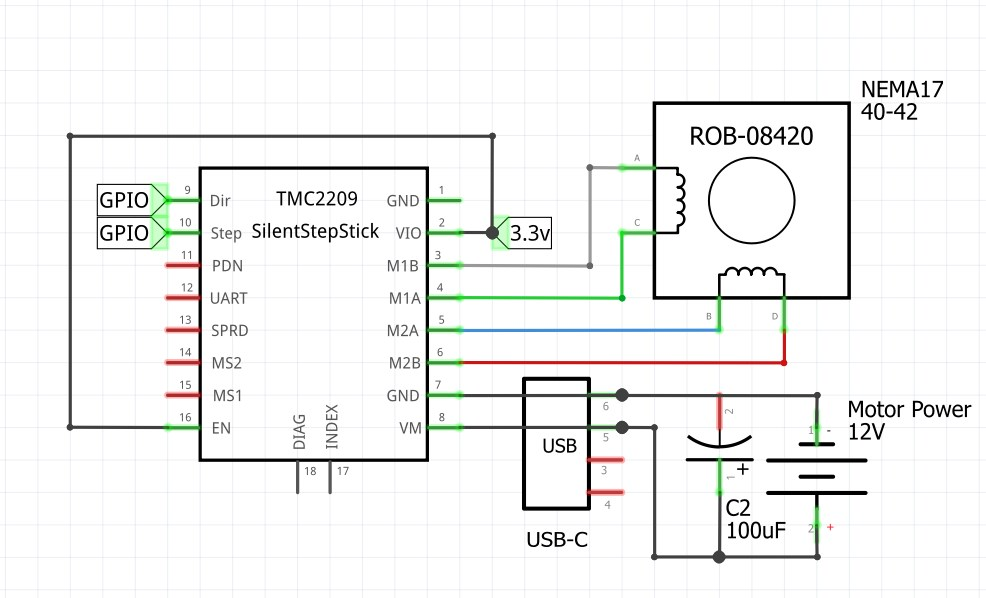
\includegraphics[width=\textwidth,height=8cm, keepaspectratio]{imgs/diagrams/tmc2209wiring.jpg}
      \caption{Schematic for NEMA17 Stepper Motor Control designed in Fritzing \cite{fritzing}}
    \end{minipage}
\end{figure}

After designing the schematic, the connections were then realised on a prototyping board, making use of the TMC2209 driver, a breakout board for a USB-C connection to provide the 12V power from the PSU, and pin headers to allow connection to the Pi and the motor.

\begin{figure}[H]
    \hfill
    \begin{minipage}[t]{0.45\textwidth}
      \centering
      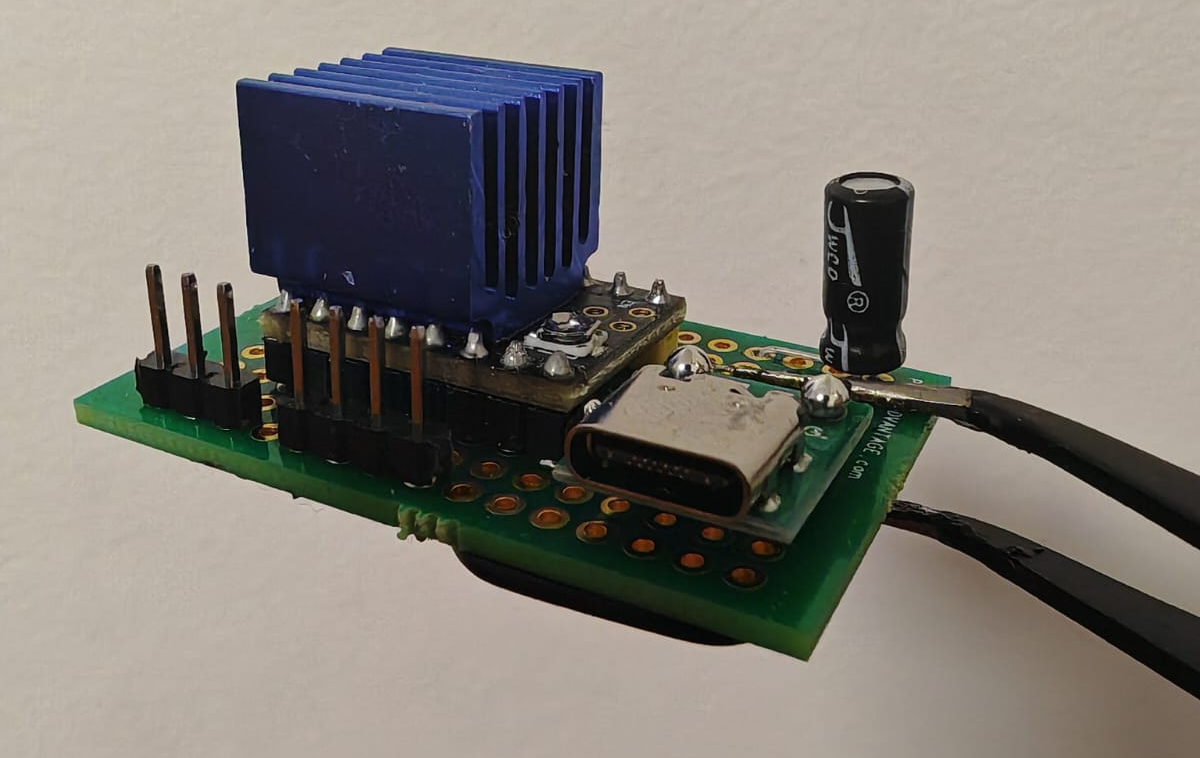
\includegraphics[width=\textwidth,height=5cm, keepaspectratio]{imgs/real/tmc2209-0.jpeg}
    \end{minipage}
    \hfill
    \begin{minipage}[t]{0.45\textwidth}
      \centering
      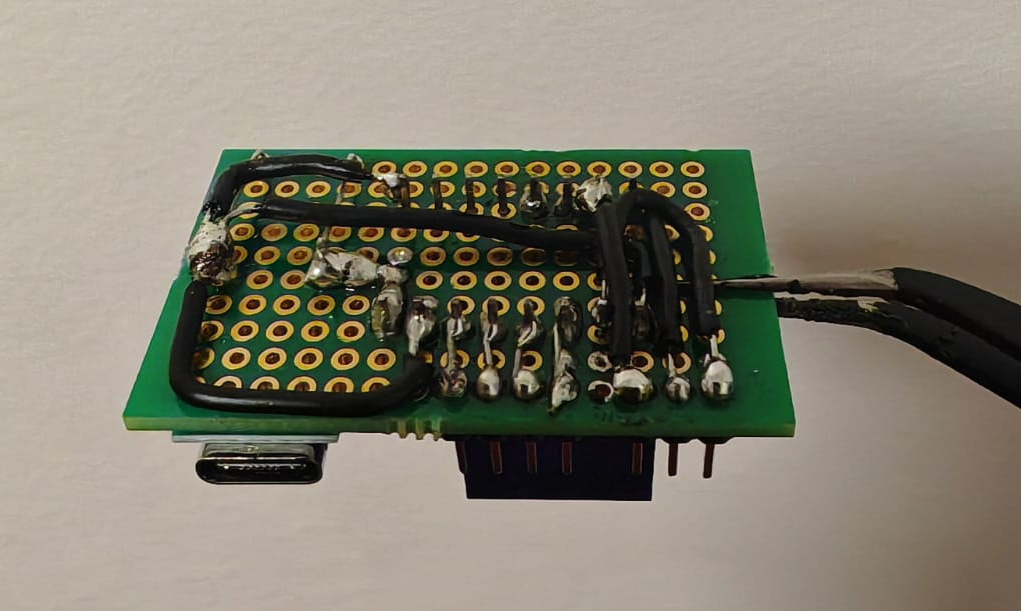
\includegraphics[width=\textwidth,height=5cm, keepaspectratio]{imgs/real/tmc2209-1.jpeg}
    \end{minipage}
    \caption{PCB for NEMA17 Stepper Motor Control}
\end{figure}

Two of these PCBs were produced due to the need for two stepper motors, and they were then connected to the Pi using the GPIO pins as shown in \autoref{tab:component-connections}.